\subsection{Noisy circuit-knitting comparison}
\label{sec:noisy-knitting}

All noisy results in this subsection are local simulations using the noise
properties and device topology encoded in
\textsc{Qiskit's} \texttt{FakeWashingtonV2} representation of the 127-qubit
\washington{} backend.  Thus ``noisy'' refers to simulation with the
Washington calibration-derived device model, not execution on the physical
device.

The \washington{} calibration is an Eagle r1-era benchmark and should not be
interpreted as the absolute noise level of current IBM hardware.  Washington
contained 127 qubits on a heavy-hex lattice.  Heron r1 increased this to 133
qubits, and Heron r2/r3 to 156 qubits, while retaining heavy-hex connectivity
and introducing fixed-frequency qubits with tunable
couplers~\cite{ibm-processor-types}.  IBM reported a
three- to five-fold device-performance improvement for Heron r1 over its
flagship Eagle processors, largely through improved two-qubit control and
suppressed crosstalk~\cite{ibm-heron-system-two}; a late-2025 Heron r3 system
reported a best error per layered gate (EPLG) of approximately
$0.23\%$~\cite{ibm-q4-2025}.  The Washington model therefore remains useful
for a controlled comparison of knitting with and without a routing
constraint, but likely overstates the absolute noise expected from current
Heron hardware.

\noindent\textit{What is compared.}\quad
Knitting changes one thing in the circuit: the two CNOTs per Trotter step
that couple the last site to the first through the periodic link are removed
and replaced by the decomposition of Sec.~\ref{sec:knitting}.  To isolate the
effect of that change, the un-knitted circuit and every knitted term are
compiled in the same way.  Both are transpiled at optimization level three,
and in both the twelve circuit qubits (six staggered sites and the six links
between them, in lattice order) are assigned to the same straight line of
twelve physical qubits of the Washington model,
$\{31,32,36,51,50,49,55,68,69,70,74,89\}$, which is the geodesic of that
length with the lowest mean calibrated CNOT error ($0.98\%$).  With this
assignment the two sites joined by the periodic link sit at the two ends of
the line, ten hops apart.  The un-knitted circuit must therefore carry that
interaction across the line with SWAP gates in every Trotter step, which is
the situation a periodic lattice faces on any processor whose connectivity
does not close the ring; the knitted terms contain no such interaction and
need no such routing.

We note that this is not what the transpiler does when left to choose the
layout.  On the heavy-hex lattice it folds the twelve-qubit ring onto a path
whose two ends are adjacent, so that the periodic link costs the un-knitted
circuit almost nothing, and in that configuration we found the knitted and
un-knitted results to agree within their uncertainties at every time.  That
escape is specific to a one-dimensional ring on a sparse lattice: the
$\mathcal{O}(L^{d-1})$ periodic links of a $d$-dimensional volume cannot all
be made adjacent, as quantified in Sec.~\ref{sec:swap}.  The pinned-line
comparison is therefore the representative one, and it is the one shown
below.

\noindent\textit{Gate counts.}\quad
Table~\ref{tab:fig7-data} lists the compiled CNOT counts of the circuits
that were run.  Before compilation the one-step circuit contains 26 CNOTs,
two of which lie on the periodic link; the two-step circuit contains 50, four
on the link.  On the line, the un-knitted one-step circuit compiles to 57
CNOTs, so 31 are routing, and the two-step circuit to $137$--$143$, of which
$87$--$93$ are routing.  Each knitted term compiles to $30$--$33$ CNOTs at one
step and $58$--$63$ at two, i.e.\ $6$--$9$ and $10$--$15$ routing CNOTs; these
remain because the hopping term couples a site to its next-nearest site
through the intervening link, which a line of qubits cannot host without a
swap.  Cutting the periodic link thus removes about half of the compiled
CNOTs at one step and $57\%$ at two.

Not every CNOT influences the measured site.  The observable is the
occupation of the central site, and only the gates in its causal cone, those
through which an error can propagate to that qubit before it is read out, can
bias it.  In the un-knitted circuit the cone contains 47 of the 57 CNOTs at
one step and 105 of the 143 at two steps; in the knitted terms it contains
$17$--$21$ of $30$--$33$ and $43$--$49$ of $58$--$63$.  Multiplying the
calibrated success probabilities of the CNOTs in the cone gives the
probability that the measured site is reached by no two-qubit error at all:
$0.65$ without knitting against $0.82$ with it at one step, and $0.32$ against
$0.62$ at two steps.  Knitting therefore roughly doubles the fraction of
noise-free two-step circuits seen by the observable.

\begin{figure*}
    \centering
    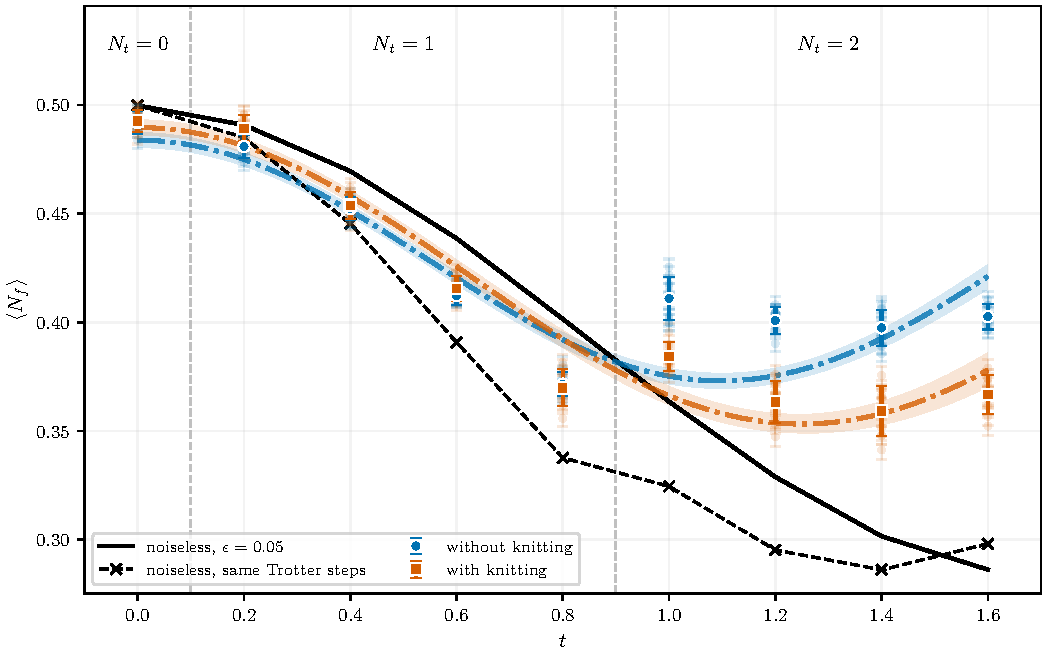
\includegraphics[width=0.98\textwidth]{figures/fermion_number_with_vs_without_knitting_scatter.pdf}
    \caption{Time evolution of the mean fermion number of the central site
    without (blue circles) and with (orange squares) circuit knitting, both
    compiled on the same straight line of twelve Washington qubits at
    optimization level three.  The solid black curve is the noiseless
    fixed-step result at $\epsilon=0.05$; the dashed black line with crosses
    is the noiseless result at the same Trotter settings as the noisy points
    (one step of size $t$, then two steps of size $t/2$), so the distance
    from a noisy point to the dashed line is the effect of noise alone.  Faint
    points are the ten individual replicas, each a run with its own simulator
    seed; the large points and error bars are the mean and standard deviation
    of a pool of $1000$ Gaussian draws per replica, each draw centred on the
    replica's value with its shot-resampling (bootstrap) width, so the error
    bar combines the shot noise within a replica with the scatter between
    replicas.  Soft dashed lines separate the regions with zero, one, and two
    Trotter steps, labeled by $N_t$.  Colored dash-dotted curves and bands
    show the truncated-cosine fits of Eq.~(\ref{eq:trunc_fit}) and their
    68\% parametric-bootstrap intervals; see the text for why these fits are
    reported but not used as mass estimates.}
    \label{fig:knitting-time-evolution}
\end{figure*}

% Generated by scripts/fit_fig7.py; do not edit by hand.
\begin{table}[t!]
\centering
\small
\begin{tabular}{c|c|c|c|c|c|c|c}\hline\hline
\multirow{2}{*}{$t$} & \multirow{2}{*}{$N_t$} & \multirow{2}{*}{$k$}
& terms
& \multicolumn{2}{c|}{$N_{\mathrm{CNOT}}$}
& \multicolumn{2}{c}{$\langle N_f\rangle$} \\ \cline{5-8}
& & & $(6^k)$ & no knit & knit & no knit & knit \\ \hline
$0.0$ & 0 & 0 & 1 & $2$ & $2$ & $0.492(5)$ & $0.493(5)$ \\ \hline
$0.2$ & \multirow{4}{*}{1} & \multirow{4}{*}{2} & \multirow{4}{*}{36} & \multirow{4}{*}{$57$} & \multirow{4}{*}{$30\text{--}33$} & $0.481(5)$ & $0.489(6)$ \\
$0.4$ &  &  &  &  &  & $0.452(5)$ & $0.454(6)$ \\
$0.6$ &  &  &  &  &  & $0.412(4)$ & $0.416(6)$ \\
$0.8$ &  &  &  &  &  & $0.372(6)$ & $0.370(9)$ \\ \hline
$1.0$ & \multirow{4}{*}{2} & \multirow{4}{*}{4} & \multirow{4}{*}{1{,}296} & \multirow{4}{*}{$137\text{--}143$} & \multirow{4}{*}{$58\text{--}63$} & $0.41(1)$ & $0.384(7)$ \\
$1.2$ &  &  &  &  &  & $0.401(6)$ & $0.36(1)$ \\
$1.4$ &  &  &  &  &  & $0.397(8)$ & $0.359(11)$ \\
$1.6$ &  &  &  &  &  & $0.403(6)$ & $0.367(9)$ \\
\hline\hline
\end{tabular}
\caption{Noisy data plotted in Fig.~\ref{fig:knitting-time-evolution} and the
associated sampling cost.  Each direct circuit and each knitted decomposition
term used $2^{14}=16{,}384$ shots for each of ten independent seeds.  The
aggregate count for each knitted data point is therefore
$N_{\mathrm{shots}}=(6^k)\mathbin{\times}10\mathbin{\times}2^{14}$; each
no-knit point has $N_{\mathrm{shots}}=10\mathbin{\times}2^{14}$.  Here
$k$ counts only the CNOTs replaced by circuit cuts, not all CNOTs in the
transpiled circuits.  The $N_{\mathrm{CNOT}}$ columns are the compiled CNOT
counts of the circuits that were run: both the direct circuit and every
knitted term are transpiled at optimization level three with the twelve
circuit qubits pinned to the same straight line of \texttt{FakeWashingtonV2}
(Sec.~\ref{sec:numresults}).  The direct range spans the ten transpiler seeds
of the un-knitted replicas; the knitted range spans all $6^k$ decomposition
terms, which share one transpiler seed.  The $t=0$ circuit contains only the
two state-preparation CNOTs.  Uncertainties are the one-standard-deviation
resampling uncertainties used in Fig.~\ref{fig:knitting-time-evolution}.}
\label{tab:fig7-data}
\end{table}


\noindent\textit{Results.}\quad
Fig.~\ref{fig:knitting-time-evolution} and Table~\ref{tab:fig7-data} compare
the two noisy series with the noiseless values at the same Trotter settings.
Noise pushes the occupation toward its fully decohered value of $1/2$ in both
cases, so the question is how much of the noiseless signal, the distance of
$\langle N_f\rangle$ from $1/2$, survives.  With one Trotter step the two
series are indistinguishable: both lie within $0.035$ of the noiseless value
at every time and within one standard deviation of each other, so at this
depth knitting neither helps nor hurts.  With two Trotter steps the
un-knitted circuit retains $48$--$51\%$ of the noiseless signal while the
knitted circuit retains $66$--$67\%$.  The un-knitted points lie
$0.086$--$0.111$ above the noiseless values and the knitted points
$0.060$--$0.073$ above them; the difference between the two series is
$0.027$--$0.038$ at each of the four two-step times, between $2.3$ and $3.3$
standard deviations individually and of the same sign at all four, and the
knitted error bars are no larger than the un-knitted ones.  The reduction in
the two-step bias, to about two thirds, is the practical benefit of cutting
the periodic link in this model; it is smaller than the factor of two in the
cone survival probability above, as expected since single-qubit, readout and
mid-circuit-measurement errors are not removed by knitting and the knitted
estimator adds the variance of the quasi-probability reconstruction.

\noindent\textit{Fits.}\quad
For completeness we fit the same nine time points in each series to
Eqs.~(\ref{eq:trunc_fit}) and~(\ref{eq:full_fit}), using the resampling
uncertainties as independent absolute weights, with parameter uncertainties
from 10,000 parametric-bootstrap replicas in which each time point is drawn
from a Gaussian with its central value and uncertainty.  The noiseless
fixed-step reference is fitted at the same nine times.  The five-parameter
form is not supported by this short window: its AICc is larger than that of
the truncated cosine and it places at least one parameter on a fit boundary
in most bootstrap replicas, so the truncated cosine is the primary model.
Table~\ref{tab:fig7-fits} reports the results.

% Generated by scripts/fit_fig7.py; do not edit by hand.
\begin{table*}[t!]
\centering
\begin{tabular}{lccccc}\hline\hline
data & $A$ & $C$ & $D$ & $\chi^2/\mathrm{dof}$ & AICc \\ \hline
noiseless, $\epsilon=0.05$ & $0.1068^{+0.0003}_{-0.0003}$ & $1.837^{+0.006}_{-0.005}$ & $0.3913^{+0.0003}_{-0.0004}$ & 25.03/6 & 35.83 \\
noisy, without knitting & $0.055^{+0.003}_{-0.003}$ & $2.86^{+0.06}_{-0.06}$ & $0.4284^{+0.0019}_{-0.0019}$ & 60.65/6 & 71.45 \\
noisy, with knitting & $0.068^{+0.003}_{-0.003}$ & $2.51^{+0.07}_{-0.08}$ & $0.421^{+0.002}_{-0.003}$ & 22.89/6 & 33.69 \\ \hline\hline
\end{tabular}
\caption{Weighted truncated cosine fits to the same nine time points shown in Fig.~\ref{fig:knitting-time-evolution}. Here $A$, $C$, and $D$ are the amplitude, frequency, and offset in Eq.~\eqref{eq:trunc_fit}. Each entry gives the bootstrap median and central 68\% parametric-bootstrap interval.}
\label{tab:fig7-fits}
\end{table*}

Using the model-selection rule described in the text, the truncated cosine is the
primary model.  The fitted knitted-minus-un-knitted frequency difference is
$\Delta C=-0.347^{+0.092}_{-0.097}$
(68\% parametric-bootstrap interval).


The truncated cosine reproduces the noiseless frequency,
$C=1.837(6)$ against $1.87$ from the long fit of
Table~\ref{tab:mass_extraction}, but it does not describe either noisy
series: $\chi^2/\mathrm{dof}=60.7/6$ without knitting and $22.9/6$ with it.
At this noise level the noisy curves flatten and turn back toward $1/2$
instead of continuing to oscillate, and the fitted $C$ values of $2.86(6)$
and $2.51(8)$ measure how quickly each curve flattens, not the meson mass.
The knitted value is closer to the noiseless one, with a difference between
the two noisy fits of $\Delta C=-0.35^{+0.09}_{-0.10}$ (95\% interval
$[-0.54,-0.17]$), consistent with the smaller bias seen point by point, but
neither series yields a mass estimate without error mitigation.  The gain
from knitting at this depth is thus in the fidelity of the time series, not
yet in a converged extraction of the mass.
